%%% TeX-command-extra-options: "-shell-escape"
% IMPORTANT: compiling from the command line using:
% pdflatex -shell-escape betaLabManual2.tex

\documentclass[a4,11pt, notitlepage]{article}

\usepackage{fixltx2e}
\usepackage[utf8]{inputenc}
\usepackage[T1]{fontenc}
\usepackage[english]{babel} 
\usepackage{graphicx}
\usepackage{textcomp}
\usepackage{mathpazo}
\usepackage{fullpage}
\usepackage{epsfig}
\usepackage{color}
\usepackage{subfigure}
\usepackage{listings}
\usepackage{SIunits}
\usepackage{rotating}
\usepackage{url}
\usepackage[hmargin=3cm,vmargin=3.5cm]{geometry}  
\usepackage{listings}

\usepackage{minted}

\begin{document} 
 

\title{\huge{Lab manual
\\KF7: $\beta$-spectrum and Fermi-Kurie plot
\\.
\\\textcolor{red}{PLEASE READ THIS DOCUMENT BEFORE COMING TO THE LAB!}}}
%\author{}
\date{\today}
\maketitle

\vspace{10pt}
\begin{abstract}
The purpose of this laboratory exercise is to determine the energy released in the process (the \textit{Q-value}) for a $\beta$-transition by studying the decay of the phosphorus isotope 
\\$^{32}P\rightarrow ^{32}S + e^- + \bar{\nu}$, and to verify Fermis Theory of the weak decay. The measurements are done by a plastic scintillation detector in combination with a multi channel analyzer, and the result is compared with the theoretically calculated value. 
\end{abstract}

\begin{figure}[htp]
  \vspace{40pt}
  \begin{center}
    
\includegraphics[width=7.0cm]{figures/LU.png}
  \end{center}
\end{figure}

\thispagestyle{empty}

\pagebreak
\tableofcontents 
\pagebreak
\section{Learning outcome}

In accordance with the syllabus of FYSC12: Nuclear Physics and Reactors, 7.5
credits, the goal of the laboration exercise is that the student -- after
completed the lab -- shall:

\begin{itemize}
\item be familiar with the basic properties of beta-decay;
\item know the main principles of how a plastic scintillator detector works;
\item be able to discuss the proper setup and procedures of the experiment;
\item with the help of the supervisor handle radioactive samples and use a
  plastic scintillator (including calibration) to measure the decay particle energy;
\item evaluate experimental results.
\end{itemize}

\section{Information}


\subsection{General}

\begin{itemize}
\item Supervisor: Hanno Perrey, office: B202
\item Email: hanno.perrey@nuclear.lu.se, please contact me for any questions regarding the lab. 
\item We start the lab 8:30 in hall L311. 
\item Bring: your laptop computer (preferably with working
  analysis setup, see below). 
\item NO FOOD or DRINKS in L311
\end{itemize}



\subsection{Prepare BEFORE the lab}

\begin{itemize}
\item Read Krane chap. 7.3, 7.6 (3 pages), 9.1, 9.2 and 9.3. 
\item Read the lab manual
\item Setup your computer to run the analysis code (see section !!!!!)
  and test it by following the first step
\end{itemize}



\subsection{Schedule}

\noindent\textbf{Morning (whole group):} 
\begin{itemize}
\item Warm-up discussion about beta decay and introduction to the
  experimental setup.
\item Collecting and analysing data to determine the $Q$ value of the
  $\beta$ decay of $^{32}$P.
\end{itemize}

\noindent\textbf{Lunch break} 

\noindent\textbf{Early afternoon (partner exercises/small groups):} 
\begin{itemize}
\item Open experiment session. Lots of unanswered questions from the
  morning: how reliable are the results, how can they be improved and
  what actually happens under the hood of our data acquisition system?
  Pick a topic to focus on and document your findings.
\end{itemize}

\noindent\textbf{Later in the afternoon (whole group):} 
\begin{itemize}
\item Concluding discussion. Present your findings and ask any
  remaining questions you might have!
\end{itemize}


\textbf{Important: }For this laboratory exercise, you \emph{do not} have to hand in any
written report. Therefore, your \emph{active} participation in the laboratory experiment is
the only and key prerequisite for a passing grade: by generally asking questions,
raising ideas for investigations, and by discussing the experiment and
its result within the group. And of course, by following your own
initiative in the afternoon when investigating a subject of your
choice (see section \ref{sec:afternoon}) and by presenting your
findings to the group during the final discussion (see section
\ref{sec:final-presentation}).

Please, do not forget to leave your feedback with the supervisor -- it
is greatly appreciate in the continued development of this exercise!

\pagebreak
\section{Introduction to laboratory exercise}

The purpose of this laboratory exercise is to measure the energy
released in the process (the \textit{Q-value}) for a
$\beta$-transition by studying the weak decay of the isotope
phosphorus-32 to sulfur ($^{32}P\rightarrow ^{32}S + e^- + \bar{\nu}$) and to compare the
resulting value to the theoretical expectation. 

For measuring the energy of the electrons from the decay, we use a
plastic scintillation detector in combination with a Multi Channel
Analyzer (MCA). Two additional radioactive sources are available for
the energy calibration of the detector.

Since the end point energy of the spectrum is experimentally difficult
to determine from the spectrum alone, the data will be analyzed by
constructing the Fermi-Kurie plot. From this, the Q-value can be
easily extracted.

Finally, we will discuss whether or not the result constitutes a
successful test of Fermi's Theory of weak decay.

\section{Brief reminder of the underlying theory}
\subsection{$\beta$-decay}

There are three different kinds of $\beta$ decay:
\begin{itemize}
\item[$\beta^-$] in this process, a neutron is converted to a proton
  with the emission of an electron and anti-neutrino,
  $n\rightarrow p + e^- + \bar \nu_e$. This decay occurs mainly for
  neutron rich nuclei; it can also happen for free neutrons.
\item[$\beta^+$] in this process, a proton is converted to a neutron
  with the emission of a positron and a neutrino,
  $p\rightarrow n + e^+ + \nu_e$. This decay occurs mainly for
  proton rich nuclei, and the proton must be bound to a nucleus.
\item[E.C.] (Electron Capture) if the energy of the excited nucleus is
  not high enough for a $\beta^{\pm}$ decay, an electron near the
  nucleus can be captured by a proton, leaving the atom in an excited
  state, where the hole is filled by an outer electron, giving
  characteristic X-rays (the energy of the X-ray is the binding energy
  of the captured electron).
\end{itemize}

\subsubsection{Q-value}

The released energy in a nuclear reaction is called the Q-value. It can be expressed as the difference in the nuclear binding energy before and after the decay: \begin{equation}
  Q_{\beta_-}=[m_{N}(X)-m_{N}(X')-m_e-m_{\nu}]\cdot c^2
\end{equation}
where $X$ is the mother nucleus, $X'$ is the daughter, and $m_N$
denote the \textit{nuclear} masses. 
%%%% !!!!!!!!!!
%%%%Calculate the Q-value for the process we are looking at in this laboratory exercise, $^{32}P\rightarrow ^{32}S + e^- + \bar{\nu}$. 


%
%\subsection{Internal conversion}
%Describe internal conversion: when the wave function of an electron from the inner shell and the nucleus wave function overlap, i.e. there is a probability for the electron to be inside the nucleus, the excited nucleus can deexcite by transfer its energy to this electron which is then emitted in a one step process (i.e. no beta decay; atomic number the same) from the atom. The vacancy makes the atom deexcite by x-ray emission when the hole is filled by an electron. OR the excitation energy is transferred to another electron which is ejected. (auger). 
%
%


\subsection{Fermi's Theory of beta decay}

In this exercise we want to determine the Q-value of phosphorus-32
decaying into sulfur. The electrons and neutrinos from this
spontaneous decay will share the Q-value as kinetic energy. The
neutrinos cannot be detected, but we can measure the kinetic energy of
the electrons and receive an energy spectrum. We can in principle
determine the Q-value from the spectrum; the highest recorded
energy. But the count rate near the end point energy is small due to
noise and background and the limited resolution of the detector, so
the value cannot be determined from the spectrum with high enough
accuracy. To calculate a better approximation of the Q-value from the
electron count rate, the Fermi Theory is used to construct a
Fermi-Kurie plot, giving us a linear function, which can be
extrapolated. The intersection with the x-axis is the Q-value; in this
way the value can be determined more precisely. In order to understand
the Fermi-Kurie plot, we have to rewrite Fermi's Golden Rule.

With
\begin{equation}
Q=T_e + T_{\nu}
\end{equation} 
and
\begin{equation}
E_e^2 = p^2c^2+m_e^2c^4=(T_e+m_ec^2)^2
\end{equation} 
we can write
\begin{equation}
Q-T_e \propto \sqrt{\frac{N(T_e)}{pE_e}} = \sqrt{\frac{N(T_e)p}{E_ef}}
\label{eq:f}
\end{equation}
where $N(T_e)$ denotes the number of electrons as function of the
electron kinetic energy, $T_e$, $f=1.3604A^2+0.1973A+0.0439$, and $A=pc/m_ec^2$ is introduced in the function to correct for the Coulomb interaction between the electron from the decay and the daughter nucleus. 
The Q-value can now easily be obtained by plotting $Q-T_e$ against $T_e$, which is the Fermi-Kurie plot.



\section{The detector and the experimental equipment}

A plastic scintillator is used for detecting the radiation. The
incident radiation interacts with the plastic molecules and excites
them. A molecule can be excited in two ways: firstly, electrons in the
atoms can be excited to higher states ($\sim 1 eV$); and secondly, the
atoms in the molecule can vibrate to higher excitations
($\sim 0.1 eV$). The molecule deexcite with the emission of visible
light, which is not energetic enough to excite further atoms; the
material is transparent to its own radiation, see Fig. \ref{fig:mol}.

\begin{figure}[htp]
  \vspace{40pt}
  \begin{center}
    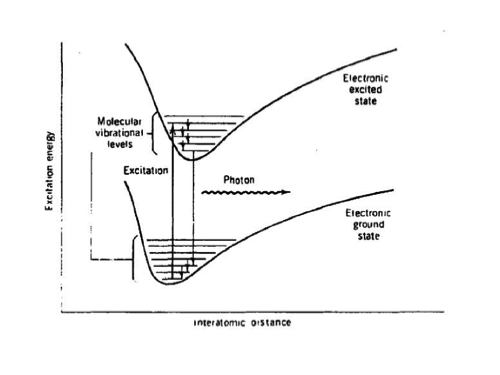
\includegraphics[width=15.0cm]{figures/Energy.png}
    \caption{Energy levels in plastic molecules.} %!!!!! REFERENCE
\label{fig:mol}
  \end{center}
\end{figure}


The light from the molecular deexcitation strikes a photocathode and
release one or more photoelectrons per photon, called
\textit{secondary electrons}, via Compton scattering. See
Fig. \ref{fig:setup} for the experimental setup. The secondary
electron are accelerated and multiplied in a photomultiplier tube
(PMT) containing dynodes at different potential. The PMT hence produce
an output voltage pulse, where the amplitude of the pulse is
proportional to the number of scintillation events, which in turn is
proportional to the energy deposited by the primary ionization. To
keep this proportionality, the transparency mentioned earlier is
necessary.

The PMT only delivers a few electrons per event. The signal therefore
needs to be amplified. Firstly, the signal is converted from a current
to a voltage pulse in the preamplifier, with a typical size of
$\sim mV$. Secondly, the pulse is amplified in the main amplifier,
where the signal go from $\sim mV$ to $\sim V$. The pulse is then
analyzed in the MCA, where it is digitized and stored in channels which
can be displayed on a computer screen.

To be able to translate the detected signal to the electron energy,
the detector must be calibrated with the help of detecting radiation
with known, discrete, energies from $^{207}Bi$ and $^{137}Cs$.

\begin{figure}[htp]
  \vspace{40pt}
  \begin{center}
    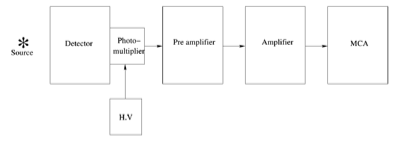
\includegraphics[width=15.0cm]{figures/Setup.png}
    \caption{The experimental setup.}
\label{fig:setup}
  \end{center}
\end{figure}

\section{Warm-up questions}

\begin{enumerate}
\item Why is $^{32}P$ a suitable sample to use in this laboratory exercise?
\item How does the electron energy spectrum look like for a $\beta^-$ decay? Why? 
\item Why must the proton undergoing $\beta^+$ decay be bound to a nucleus?
\item Calculate the Q-value for the process $^{32}P\rightarrow ^{32}S + e^- + \bar{\nu}$. Hint: you can neglect the neutrino mass and the difference in binding energy of the electrons, why? 
\item Why can we neglect the recoil energy of the daughter particle?
\item By what mechanisms does a photon/charged particle lose energy
  when traversing material?
\item Why is plastic a good material for a scintillator?
\end{enumerate}


\section{The morning: measure $Q$ value of the $\beta$ decay of $^{32}$P}
This part of the laboratory exercise is going to be ``guided'' yet
interactive. Please see section \ref{sec:prerequisites} for what you
need to run the analysis on your own computer as we go through the measurement steps.

This is the rough outline:
\begin{enumerate}
\item Measure $^{32}P$
  \begin{itemize}
  \item Discuss: How long should the measurement run? Does the spectra
    look as expected? Is this all we need to determine $Q$?
  \end{itemize}
\item Measure some more?
  \begin{itemize}
  \item $^{137}$Cs?
  \item $^{207}$Bi?
  \item add shielding to the above?
  \item leave the source out completely?
  \end{itemize}
\item Analyse the results!
  \begin{itemize}
  \item Plot the measured data
  \item Calibrate the detector
  \item Correct data for background
  \end{itemize}
\item Construct the Fermi-Kurie plot and determine $Q$
\item Discuss the result and compare to expectation -- and where to go
  from here?
\end{enumerate}

\subsection{Data Analysis}
\label{sec:data-analysis}

The ``online'' visualization that the Maestro MCA software allows is
very helpful but limited and tedious to use for multiple data samples
-- no way around writing our own code!

Lucky for you, pretty much the whole analysis is already coded and
uploaded to
\url{https://bitbucket.org/hperrey/betalab_analysis}. The next
sections explain what is needed in order to run the analysis and how
to do so.

\subsubsection{Prerequisites}
\label{sec:prerequisites}

The analysis is written in Python with the SciPy tools for scientific
computing -- it's all open-source, doesn't cost anything, available
for all major platforms and highly flexible; the key packages are just
a download away, just follow the instructions at: \url{http://www.scipy.org/install.html}

If you want to hack around the code, it might be useful to install
\texttt{git} as well, a source-code version control tool (never to
early to learn git$\ldots$): \url{https://git-scm.com/}

\subsubsection{Running the analysis}
\label{sec:running-analysis}

Download the code from
\url{https://bitbucket.org/hperrey/betalab_analysis} into a directory
of your liking or clone the whole repository with \texttt{git} by running
\begin{minted}[mathescape]{bash}
git clone https://bitbucket.org/hperrey/betalab_analysis
\end{minted}

Use a text editor of your choice (or ask the supervisor for
recommendations) and open the file \texttt{analysis.py}. Find the part
where the data file is opened and plotted. Adjust the path to your own
data if needed.

Now enter the directory and actually run the central analysis by executing \texttt{analysis.py} e.g. by
entering
\begin{minted}[mathescape]{bash}
python3 analysis.py
\end{minted}
in a terminal.

\subsubsection{Energy calibration}
\label{sec:energy-calib}

Some information that might be useful to extend the energy
calibration: Table \ref{tab:calib} shows the energies of electrons released from
internal conversion for bismuth-207 and the relative intensities.

\begin{table}[h]
\caption{Energies and relative intensities for internal conversion
  electrons of $^{207}$Bi (useful information in the detector calibration).}
\label{tab:calib}
\centering
\begin{tabular}{ccc}
Shell & $E_{e}$ (MeV) & I \\
$K_1$ & 0.483 & 1.55 \\
$L_1$ & 0.555 & 0.45 \\
$M_1$ & 0.568 & 0.15 \\
$K_2$ & 0.976 & 7.05 \\
$L_2$ & 1.049 & 1.85 \\
$M_2$ & 1.062 & 0.60 
\end{tabular}
\end{table}


\section{The afternoon: a choice of further studies}
\label{sec:afternoon}

\begin{itemize}
\item Prepare to report your findings \emph{in a way that the
    whole group can understand}: what have you been doing, and why?
  What to make of your result? How does it tie in with the experiment
  and with the activities of the others?
\item Feel free to give this a personal touch and to diverge on things
  you have discovered or learned along the way -- the presentation
  will be informal in style.
\item Keep notes! Make pictures! Think of a joke to tell!
\item If you don't finish the project or something does not work:
  don't worry! That's life as an (experimental) physicist... Document
  your findings and explain what went wrong to your colleagues so that
  they (or you) don't make the same mistake again.
\item There is overlapp between the different topics -- embrace it and
  discuss among your colleagues!
\end{itemize}

\subsection{Uncovering Uncertainties}
\label{sec:uncertainties}

In order to interpret any measurement result, one has to fully
understand the associated systematical (and statistical)
uncertainties.

\noindent\textbf{Mission:} Quantify the uncertainty of the $Q$ value measurement.

\noindent\textbf{Hints:}
\begin{itemize}
\item What are \emph{possible} sources of systematic uncertainties?
  Which ones are actually \emph{likely}?
\item Which sources of uncertainty do you expect to contribute the most?
\item How can you access these sources of uncertainties? I.e. by what
  method/variation could you estimate their impact?
\item Take measurements, document the effects
\item Use the analysis code to run variation of the input data through
  -- what is the effect on the final result?
\item By what systematic procedure could one estimate the dominating
  uncertainties and quantify them? Try it!
\item How do your colleagues investigations tie into systematic
  uncertainties of the experiment?
\end{itemize}


\subsection{Calibrate for better results}
\label{sec:calibrate}

Any detector is only as good as its calibration. By improving the
method and/or using additional data points in the calibration, we can
improve on the accuracy of the measurement (and get a handle on the
uncertainties associated with the calibration).

\noindent\textbf{Mission:} Improve the energy calibration of the experimental setup.

\noindent\textbf{Hints:}
\begin{itemize}
\item There is another source with known peaks from internal
  conversion electrons available to collect data from: bismuth-207
  ($^{207}$Bi).
\item Are you satisfied with the data from $^{137}$Cs?
\item How can the peaks be more precisely determined?
\item Does the background subtraction work as expected?
\item Are all data points (i.e. peaks) equally precise? How could you
  weight their impact on the calibration?
\item Should you exclude some points from the data?
\item What is the impact on the calibration (and the $Q$ value) if you
  vary the input data and/or method?
\item In an ideal laboratory, how would you want to improve the
  calibration further?
\end{itemize}

\subsection{One person's background is another one's data}
\label{sec:background}

\noindent\textbf{Mission:} Using plastic scintillator detectors, study the
background due to cosmics.

\noindent\textbf{Hints:}
\begin{itemize}
\item There are two large pedal plastic scintillators with PMTs
  available -- use this as cosmic ray detector. What geometric
  arrangement is best suited for such a measurement?
\item \textbf{Important:} Before moving or connecting the pedal detectors to HV, consult
  the supervisor and discuss the necessary steps with them! The PMTs
  can only take negative (-) 1500V \emph{maximum}. Do not go beyond
  -1300V before discussing this with the supervisor!
\item We have several NIM electronic modules to construct a simple
  counter with: discriminators, coincidence logic, and visual
  scaler. Research how these function and how to connect them together.
\item Use a scope to study the signals coming from the scintillators;
  what do they look like and how do they vary from a source's signal?
  What is the energy that we expect from cosmics?
\item Determine the count rate and estimate the rate seen in the
  detector used for measuring the $Q$ value -- how much do cosmics
  contribute to the background and over what energy region? What could
  one do to shield them?
\end{itemize}

\subsection{Open-signal surgery}
\label{sec:}
For the measurements performed in the morning, we used an MCA to
give us pulse-height spectra. However, what do the signals from the
actual detector look like that yielded these spectra?

\noindent\textbf{Mission:} Connect a scope to the PMT and study its
signals. Try to understand what you see.

\noindent\textbf{Hints:}
\begin{itemize}
\item The scope supports to save waveforms/images -- a good way to
  keep record of your findings.
\item Trigger on signals of various heights; does their shape change
  at all?
\item Can you relate what you see to
the spectra we measured?
\item Do you notice anything unusual? Save those waveforms! What could
  be the origin?
\item How do the signals change with source? Or with high-voltate to the
  PMT? (\textbf{Attention:} Do not change the HV before consulting
  your supervisor!
\item Do you notice any electronic noise? How do the pre-amp settings
  influence this?
\end{itemize}


\section{Late afternoon: Concluding discussion and presentation of findings}
\label{sec:final-presentation}

\begin{itemize}
\item Motivate your steps -- what provides your project to the experiment?
\item Keep it simple -- everyone should understand and follow what you
  have been doing.
\item Try to relate what you have learned to the projects of
  others.
\item Stay away from any presentation software -- think more
  show-and-tell/whiteboard/simple picture show instead of elaborate slide show.

\end{itemize}

\appendix

\section{Final discussion points}
\label{sec:further-discussion}

Teachers notes/suggestions only -- ask away if you wish!

\begin{itemize}
\item What have we learned more since the measurements this morning?
\item Were any of the results particularly surprising for you?
\item Are we now ready to publish the results? What would we have to
  do further?
\item With all we know now, what would you do to improve the
  experiment? Where do you see limiting factors to its precision?
\end{itemize}

\pagebreak
\section{Feedback}
\label{sec:feedback}

Please fill out the following set of questions and hand them in
(anonymously) to the supervisor. Feel free to leave the manual as a
whole should you have noted any corrections/suggestions in it!

\begin{itemize}
\item What was your favorite part of the lab exercise?
\vspace{3cm}

\item What was your least favorite part? Why?
\vspace{3cm}

\item What information would liked to have had \emph{before} the lab?
\vspace{3cm}

\item What information did you miss \emph{during} the lab?
\vspace{3cm}

\item What do you feel you have learned from the lab?
\vspace{3cm}

\item Any more comments or suggestions?
\vspace{5cm}

\end{itemize}

\end{document}


